\chapter{Современные системы управления}

Современные технологические процессы повышают требования для качества управления. Исследователи применяют для решения задач в данной области множество методов, в том числе искусственные нейронные сети, имеющие высокий потенциал в этой области. Однако они не обеспечивают значимых преимуществ перед классическими подходами и требуют улучшения.
В данной главе рассматриваются современные технологии и методы, применяемые в системах управления технологическими процессами, оценивается их эффективность и недостатки. Определены исходные данные для анализа и параметры качества. Выполнена постановка задачи исследования.

\section{ПИД-регуляторы}

ПИД-регуляторы доказали свою эффективность в управлении разнообразными процессами. Их использование не требует знания точной модели процесса, поэтому они эффективны в управлении промышленными и технологическими процессами, математические модели которых достаточно сложно определить. ПИД-регуляторы строятся на основе классической теории управления и просты для понимания и реализации (рис. \ref{fig:PID_controller_scheme}).
\begin{figure}[H]
    \centering
    	\begin{tikzpicture}[scale=0.6]
    	\node at (0,5) {\fontsize{6}{0}\selectfont задание};
    	\draw[->] (0.8,5) -- (2.4,5);
    	%отрисовка сумматора и стрелки от него
    	\draw (3,5) circle [radius=0.5cm];
    	\node at (2.7,5.8) {\fontsize{6}{0}\selectfont +};
    	\node at (2.7,4.2) {\fontsize{6}{0}\selectfont -};
    	\node at (3,5) {\fontsize{8}{0}\selectfont$\sum$};
    	\draw[->] (3.6,5) -- (5,5);
    	\node at (6,5){\fontsize{6}{0}\selectfont ошибка};
    	%отрисовка линий после "ошибка"
    	\draw[->] (6.8,5) -- (8,5);
    	\draw (6,5.2) -- (6,7);
    	\draw[->] (6,7)--(8,7);
    	\draw (6,4.8) -- (6,3);
    	\draw[->] (6,3)--(8,3);
    	%отрисовка PID блоков
    	\draw (8.2,6.25) rectangle(12,7.75);
    	\draw (8.2,4.25) rectangle(12,5.75);
    	\draw (8.2,2.25) rectangle(12,3.75);
    	\node at (10,7){\fontsize{8}{0}\selectfont $P\ \ \ \ \ \ \ K_p e(t)$};
    	\node at (10,5){\fontsize{8}{0}\selectfont$I\ \ K_i \int e(t) \,{d}x$};
    	\node at (10,3){\fontsize{8}{0}\selectfont$D \ \ \ \ \ \ \ \ \ K_d\frac{\partial e}{\partial t}$};
    	%Отрисовка стрелочек и сумматора после PID блоков
    	\draw (14,5) circle [radius=0.5cm];
    	\node at (14,5) {\fontsize{8}{0}\selectfont$\sum$};
    	\draw(12.2,7)--(14,7);
    	\draw [->](14,7)--(14,5.7);
    	\draw [->](12.2,5)--(13.4,5);
    	\draw(12.2,3)--(14,3);
    	\draw [->](14,3)--(14,4.4);
    	%отрисовка блока процесса, выхода и стрелочек от них
    	\draw [->](14.6,5)--(15.6,5);
    	\draw (15.8,4.25) rectangle(19.6,5.75);
    	\node at (17.7,5){\fontsize{8}{0}\selectfont процесс};
    	\draw[->](19.7,5)--(20.2,5);
    	\node at (21,5){\fontsize{6}{0}\selectfont выход};
    	\draw[->](21.7,5)--(22.5,5);
    	\draw (21,4.8)--(21,1.5);
    	\draw (21,1.5)--(3,1.5);
    	\draw[->](3,1.5)--(3,4.4);
    \end{tikzpicture}
    
    \caption{Структурная схема ПИД-регулятора}
    \label{fig:PID_controller_scheme}
\end{figure}

\subsection{Описание ПИД-регуляторов}

Назначение ПИД-регулятора – в поддержании заданного значения $x_0$ некоторой величины $x$ с помощью изменения другой величины $u$. Значение $x_0$ называется заданием, а разность $e = (x_0 - x)$ – невязкой или рассогласованием. Выходной сигнал контроллера $u$ определяется тремя слагаемыми:

\begin{equation}
    \label{eq_PID}
    u(t) = P + I + D = K_P e(t) + K_I \int_{0}^{t} e(t) dt + K_D \frac{de}{dt}
\end{equation}

где $K_P, K_I, K_D$ – коэффициенты усиления пропорциональной, интегральной и дифференциальной составляющих контроллера, соответственно.
Большинство методов настройки ПИД-регулятора используют несколько иную формулу для выходного сигнала, в которой на пропорциональный коэффициент усиления умножены также интегральная и дифференциальная составляющие:

\begin{equation}
    u(t) = K_P \left( e(t) + \frac{1}{T_I} \int_{o}^{t} e(\tau) d \tau +T_D \frac{de}{dt}\right).
\end{equation}

\textbf{Пропорциональная составляющая} – $K_P$ – вырабатывает выходной сигнал, который стабилизирует отклонение регулируемой величины. Выходной сигнал пропорциональной составляющей тем больше, чем сильнее регулируемая величина отклоняется от задания. Если входной сигнал равен заданию, то выходной равен нулю.

При использовании пропорционального контроллера значение регулируемой величины никогда не стабилизируется на заданном значении. Существует так называемая статическая ошибка, которая равна такому отклонению регулируемой величины, которое обеспечивает выходной сигнал, стабилизирующий выходную величину именно на этом значении. Например, в контроллере температуры выходной сигнал (мощность нагревателя) постепенно уменьшается при приближении температуры к заданию, и система стабилизируется при мощности равной тепловым потерям. Температура не может достичь задания, так как в этом случае мощность нагревателя станет равна нулю, и он начнет остывать.

Чем больше коэффициент пропорциональности между входным и выходным сигналом (коэффициент усиления), тем меньше статическая ошибка, однако при слишком большом коэффициенте усиления могут начаться автоколебания, а при дальнейшем увеличении коэффициента система может потерять устойчивость.

Для устранения статической ошибки используют \textbf{интегральную составляющую} – $K_I$. Она позволяет регулятору «учиться» на предыдущем опыте. Если система не испытывает внешних возмущений, то через некоторое время регулируемая величина стабилизируется на заданном значении, сигнал пропорциональной составляющей будет равен нулю, а выходной сигнал будет полностью обеспечивать интегральная составляющая.

\textbf{Дифференциальная составляющая} – $K_D$ – противодействует предполагаемым отклонениям регулируемой величины, которые могут произойти в будущем. Эти отклонения могут быть вызваны внешними возмущениями или запаздыванием воздействия регулятора на систему. Чем быстрее регулируемая величина отклоняется от задания, тем сильнее противодействие, создаваемое дифференциальной составляющей.

\subsection{Достоинства и недостатки ПИД-регуляторов}

Установление связей между параметрами и управление действиями системы может осуществляться инженерами-практиками и операторами.
Кроме того, за последние десятилетия разработано несколько методов настройки ПИД-регуляторов.

Однако, наряду с вышеуказанными достоинствами, ПИД-регуляторы имеют и ряд недостатков. Так, если рабочая точка процесса изменяется из-за возмущений, параметры контроллера требуется перенастраивать вручную, чтобы получить новую оптимальную настройку. Настройка должна осуществляться опытным оператором. Для систем с взаимодействующими контурами это процедура может быть сложной и занимать много времени. Кроме того, для процессов с переменными параметрами, временными задержками, существенными нелинейностями и значительными помехами использование ПИД-регуляторов может не обеспечить оптимальных характеристик.

Методы настройки ПИД-регуляторов также имеют ряд недостатков.
Одна из идей повышения эффективности ПИД-регуляторов заключается в управлении с самонастройкой, в котором параметры контроллера настраивались бы в оперативном режиме.

\subsection{Дискретная реализации ПИД-регулятора}

Идеализированное уравнение ПИД-регулятора (\ref{eq_PID}) является непрерывным, т. е. использует непрерывное время. При построении регулятора на базе компьютера входные и выходные переменные регулятора необходимо квантовать по времени с некоторым шагом $T_0$, и преобразовать в цифровую форму с помощью аналого-цифровых и цифро-аналоговых преобразователей. При этом уравнение ПИД-регулятора должно быть преобразовано в разностное с помощью замены производных конечной разностью, а интеграла – конечной суммой. В зависимости от выбранного метода перехода от непрерывных операторов к их дискретным аналогам возникает несколько различных уравнений, описывающих дискретные ПИД-регуляторы. При использовании метода прямоугольников для замены интеграла конечной суммой получим \cite{PID_NIL_AP}:


\begin{equation}\label{eq_discrete_PID}
    u_k = K\left[ e_k + \frac{T_0}{T_I} \sum_{i = 0}^{k} {e_{i - 1}} + \frac{T_D}{T_0} (e_k - e_{k - 1})\right],
\end{equation}

где $k = 0, 1, \ldots\frac{t}{T_0}$ - порядковый номер отсчета дискретного времени.

Недостатком такого представления уравнения регулятора является необходимость помнить значения отклонений $e_k$ для всех моментов времени от начала процесса регулирования.

Этот недостаток можно устранить, если для вычисления текущего значения управляющей переменной $u_k$ использовать ее предыдущее значение $u_{k - 1}$ и поправочный член. Для получения такого рекуррентного алгоритма достаточно вычесть из уравнения (\ref{eq_discrete_PID}) следующее уравнение \cite{PID_NIL_AP}:

\begin{equation}
        u_{k - 1} = K \left[e_{k - 1} + \frac{T_0}{T_I} \sum_{i=0}^{k-1}{e_{i - 1}}+\frac{T_D}{T_0}(e_{k - 1} - e_{k - 2})\right].
\end{equation}

В результате получим [6]:

\begin{equation}
    u_k - u_{k - 1} = q_0 e_k + q_1 e_{k - 1} + q_2 e_{k - 2},
\end{equation}

Где

\begin{equation}
    q_0=\mathbf{K}\left(1+\frac{T_D}{T_0}\right),
\end{equation}

\begin{equation}
    q_1=-\mathbf{K}\left(1+2\frac{T_D}{T_0}-\frac{T_0}{T_I}\right),
\end{equation}

\begin{equation}
    q_2=\mathbf{K}\frac{T_D}{T_0}.
\end{equation}

Таким образом, для вычисления текущего значения управляющего воздействия $u_k$ на объект управления достаточно хранить в памяти только величины $u_{k - 1}$, $e_k$, $e_{k - 1}$, $e_{k - 2}$.

Итак, алгоритм работы ПИД-регулятора может быть представлен в следующем виде [3]:

\begin{equation}\label{PID_algorithm}
    \begin{gathered}
    u_k = u_{k - 1} + \Delta u_k, \\
    \Delta u_k = q_0 e_k + q_1 e_{k - 1} + q_2 e_{k - 2}, \\
    q_0 = \mathbf{K}\left(1 + \frac{T_D}{T_0}\right), q_1 = -\mathbf{K}\left(1 + 2\frac{T_D}{T_0} - \frac{T_0}{T_I}\right), q_2 = \mathbf{K}\frac{T_D}{T_0}.
    \end{gathered}
\end{equation}

При переходе от непрерывных операторов к дискретным возникает погрешность, величина которой пропорциональна остаточному члену ряда Тейлора функции $e\left(t\right)$. Поэтому полученные дискретные уравнения можно считать эквивалентными непрерывным только при условии, что $e\left(t\right)$ изменяется слабо в пределах такта квантования. Однако с помощью аппарата z-преобразования можно показать, что основные свойства ПИД-регулятора сохраняются и при больших шагах квантования, если параметры регулятор $q_0$, $q_1$, $q_2$ выбирать не на основании параметров его непрерывного аналога, а независимо от них, методами параметрической оптимизации, выбрав необходимый критерий качества оптимизации исходя из цели регулирования. Такт квантования выбирают аналогично \cite{PID_NIL_AP}.

\section{Нейроуправление}

Нейроуправление – одно из основных направлений применения искусственных нейронных сетей. Для того чтобы алгоритмы управления могли применяться на практике, они должны быть достаточно простыми для реализации и понимания, обладать способностью к обучению, гибкостью, устойчивостью, нелинейностью. Таким образом, нейронные сети из-за своей способности обучаться на основе соотношения «вход-выход», нелинейными обобщающими способностями пригодны для решения задач управления, которые принципиально связаны с нелинейными характеристиками.

\subsection{Нейронные сети как основа построения нейрорегуляторов}

Несмотря на большое разнообразие вариантов нейронных сетей, все они имеют общие черты. Так, все они, так же, как и мозг человека, состоят из большого числа связанных между собой однотипных элементов – нейронов, которые имитируют нейроны головного мозга (рис. \ref{fig:neuron_scheme}).

\begin{figure}[H]
    \centering
    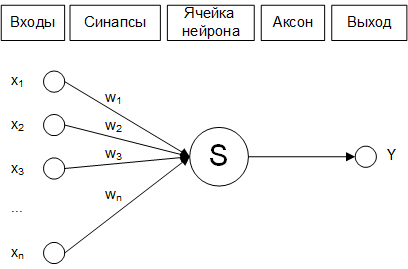
\includegraphics{images/chapter_1/Схема нейрона.png}
    \caption{Схема нейрона}
    \label{fig:neuron_scheme}
\end{figure}

Из рисунка видно, что искусственный нейрон, так же, как и живой, состоит из синапсов, связывающих входы нейрона с ядром; ядра нейрона, которое осуществляет обработку входных сигналов и аксона, который связывает нейрон с нейронами следующего слоя. Каждый синапс имеет вес, который определяет, насколько соответствующий вход нейрона влияет на его состояние. Текущее состояние нейрона определяется, как взвешенная сумма его входов:

\begin{equation}
    s = \sum_{i=1}^{n}{x_i w_i}.
\end{equation}

Выход нейрона есть функция его состояния:

\begin{equation}
    y = f(s).
\end{equation}

Нелинейная функция f называется функцией активации и может иметь различный вид (рис. \ref{fig:neuron_activation_functions}).

\begin{figure}[H]
    \centering
    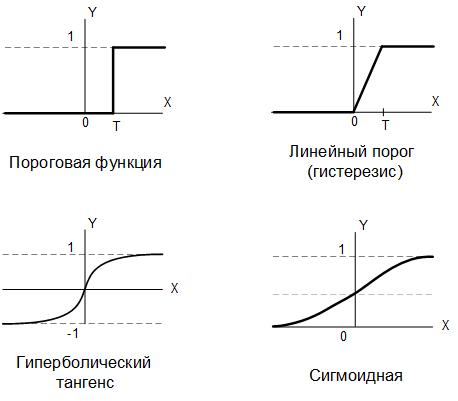
\includegraphics{images/chapter_1/Функции активации нейронов.png}
    \caption{Функции активации}
    \label{fig:neuron_activation_functions}
\end{figure}

Одной из наиболее распространенных является нелинейная функция с насыщением, так называемая сигмоидная функция:

\begin{equation}
    f(x) = \frac{1}{1 + e^{-\alpha x}}.
\end{equation}

Возвращаясь к общим чертам, присущим всем НС, отметим принцип параллельной обработки сигналов, который достигается путем объединения большого числа нейронов в так называемые слои и соединения определенным образом нейронов различных слоев, а также, в некоторых конфигурациях, и нейронов одного слоя между собой, причем обработка взаимодействия всех нейронов ведется послойно. В качестве примера простейшей НС рассмотрим трехнейронный персептрон (рис. \ref{fig:neuron_3x}), то есть такую сеть, нейроны которой имеют пороговую активационную функцию.

\begin{figure}[H]
    \centering
    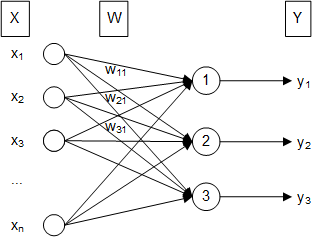
\includegraphics{images/chapter_1/Трехнейронный персептрон.png}
    \caption{Однослойный персептрон}
    \label{fig:neuron_3x}
\end{figure}

На $n$ входов поступают некие сигналы, проходящие по синапсам на $3$ нейрона, образующие единственный слой этой НС и выдающие три выходных сигнала:

\begin{equation}
    y_j = f\left[\sum_{i=1}^{n}{x_i w_{i j}}\right], j = 1..3.
\end{equation}

Очевидно, что все весовые коэффициенты синапсов одного слоя нейронов можно свести в матрицу $W$, в которой каждый элемент $w_{i j}$ задает величину $i$-ой синаптической связи $j$-го нейрона. Таким образом, процесс, происходящий в НС, может быть записан в матричной форме:

\begin{equation}
    Y = F(X W),
\end{equation}

где $X$ и $Y$ – соответственно входной и выходной сигнальные векторы, $F(V)$ – активационная функция, применяемая поэлементно к компонентам вектора $V$.

Теоретически число слоев и число нейронов в каждом слое может быть произвольным. Подробно рассмотрим алгоритм обучения многослойных нейронных сетей – алгоритм обратного распространения ошибки.

\subsection{Математические основы алгоритма обратного распространения ошибки}

\textbf{Алгоритм обратного распространения ошибки} является эффективным средством для обучения многослойных нейронных сетей.

Рассмотрим нейронную сеть, состоящую из четырех слоев (рис. \ref{fig:neural_network_4x}).

\begin{figure}[H]
    \centering
    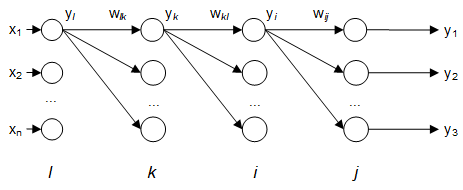
\includegraphics{images/chapter_1/Четырехслойная нейронная сеть.png}
    \caption{Четырехслойная нейронная сеть}
    \label{fig:neural_network_4x}
\end{figure}

Обозначим слои нейронных элементов от входа к выходу соответственно через $l$, $k$, $i$, $j$. Тогда выходное значение $j$-го нейрона последнего слоя равняется:

\begin{equation}
    y_j = F(S_j),
\end{equation}

\begin{equation}
    S_j = \sum_{i}{\omega_{i j} y_i - T_j},
\end{equation}

где $S_j$ — взвешенная сумма $j$-го нейрона выходного слоя; $y_i$ — выходное
значение $i$-го нейрона предпоследнего слоя; $\omega_{i j}$ — соответственно весовой коэффициент и порог $j$-го нейрона выходного слоя.

Аналогичным образом выходное значение $i$-го нейрона предпоследнего слоя определяется как:

\begin{equation}
    y_i = F(S_i),
\end{equation}

\begin{equation}
    S_i = \sum_{k}{\omega_{k i} y_k - T_i},
\end{equation}

Соответственно для $k$-го слоя:

\begin{equation}
    y_k = F(S_k),
\end{equation}

\begin{equation}
    S_k = \sum_{l}{\omega_{l k} x_l - T_k}.
\end{equation}

Алгоритм обратного распространения ошибки минимизирует среднеквадратичную ошибку нейронной сети. Для этого с целью настройки синаптических связей используется метод градиентного спуска в пространстве весовых коэффициентов и порогов нейронной сети. Согласно методу градиентного спуска изменение весовых коэффициентов и порогов нейронной сети происходит по следующему правилу:

\begin{equation}
    \omega_{i j}(t + 1) = \omega_{i j}(t) - \alpha\frac{\partial E}{\partial\omega_{i j}(t)},
\end{equation}

\begin{equation}
    T_j(t + 1) = T_j(t) - \alpha\frac{\partial E}{\partial T_j(t)},
\end{equation}

где $E$ — среднеквадратичная ошибка нейронной сети для одного образа.

Она определяется, как

\begin{equation}
    E = \frac{1}{2} \sum_{j}{(y_j - t_j)^2},
\end{equation}

где $t_j$ — эталонное выходное значение $j$-го нейрона.

Ошибка $j$-го нейрона выходного слоя равняется:

\begin{equation}
    \gamma_j = y_j - t_j.
\end{equation}

\textbf{Теорема.} Для любого скрытого слоя $i$ ошибка $i$-го нейронного элемента определяется рекурсивным образом через ошибки нейронов следующего слоя $j$:

\begin{equation}
    \gamma_i = \sum_{j = 1}^{m}{\gamma_j F^\prime(S_j)\omega_{i j},}
\end{equation}

где $m$ — количество нейронов следующего слоя по отношению к слою $i$; $\omega_{i j}$ — синаптическая связь между $i$-м и $j$-м нейроном различных слоев; $S_j$ — взвешенная сумма $j$-го нейрона.

\textbf{Теорема.} Производные среднеквадратичной ошибки по весовым коэффициентам и порогам нейронных элементов для любых двух слоев $i$ и $j$ многослойной сети определяются следующим образом:

\begin{equation}
    \frac{\partial E}{\partial\omega_{i j}} = -\gamma_j F^\prime(S_j) y_i,
\end{equation}

\begin{equation}
    \frac{\partial E}{\partial T_j} = \gamma_j F^\prime(S_j).
\end{equation}

\textbf{Следствие:} для минимизации среднеквадратичной ошибки сети весовые коэффициенты и пороги нейронных элементов должны изменяться с течением времени следующим образом:

\begin{equation}
    \omega_{i j}(t + 1) = \omega_{i j}(t) - \alpha\gamma_jF^\prime(S_j) y_i,
\end{equation}

\begin{equation}
    T_j(t + 1) = T_j(t) + \alpha\gamma_jF^\prime(S_j),
\end{equation}

где $\alpha$ — скорость обучения.

Данное следствие является очевидным. Оно определяет правило обучения многослойных нейронных сетей в общем виде, которое называется \textbf{обобщенным дельта правилом \cite{Golovko_2001}}.

\subsection{Обобщенное дельта правило для сигмоидной функции активации нейронных элементов}

Выходное значение $j$-го нейронного элемента определяется следующим образом:

\begin{equation}
    y_j = \frac{1}{1 + e^{-S_j}},
\end{equation}

\begin{equation}
    S_j = \sum_{i} {\omega_{i j} y_i - T_j}.
\end{equation}

Тогда:

\begin{equation}
    F^\prime(S_j) = \frac{\partial y_j}{\partial S_j} = y_j(1 - y_j).
\end{equation}

В результате обобщенное дельта правило для сигмоидной функции активации можно представить в следующем виде:

\begin{equation}
    \omega_{i j}(t + 1) = \omega_{i j}(t) - \alpha\gamma_j y_j (1 - y_j) y_i,
\end{equation}

\begin{equation}
    T_j(t + 1) = T_j + \alpha\gamma_j y_j(1 - y_j).
\end{equation}

Ошибка для $j$-го нейрона выходного слоя определяется, как:

\begin{equation}
    \gamma_j = y_j - t_j.
\end{equation}

Для $j$-го нейронного элемента скрытого слоя:

\begin{equation}
    \gamma_j = \sum_{i = 1}^{m}{\gamma_i y_i(1 - y_i)\omega_{j i},}
\end{equation}

где $m$ – количество нейронных элементов следующего слоя по отношению к слою $i$ (рис. \ref{fig:neuron_error}).

\begin{figure}[H]
    \centering
    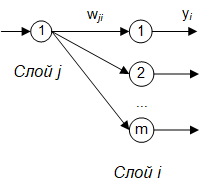
\includegraphics{images/chapter_1/Определение ошибки j-го нейронного элемента.png}
    \caption{Определение ошибки $j$-го нейронного элемента}
    \label{fig:neuron_error}
\end{figure}

\subsection{Алгоритм обратного распространения ошибки}

Как уже отмечалось, алгоритм обратного распространения ошибки был предложен в 1986 г. рядом авторов независимо друг от друга. Он является эффективным средством обучения нейронных сетей и представляет собой следующую последовательность шагов:

\begin{enumerate}[wide, labelindent=10mm]
    \item Задается шаг обучения $\alpha$ $(0 < \alpha < 1)$ и желаемая среднеквадратичная ошибка нейронной сети $E_m$.

    \item Случайным образом инициализируются весовые коэффициенты и пороговые значения нейронной сети.

    \item Последовательно подаются образы из обучающей выборки на вход нейронной сети. При этом для каждого входного образа выполняются следующие действия:

    \begin{enumerate}[wide, labelindent=20mm]
        \item производится фаза прямого распространения входного образа по нейронной сети. При этом вычисляется выходная активность всех нейронных элементов сети:

        \begin{equation}
            y_j = F(\sum_{i}{\omega_{i j}y_i - T_j)}.
        \end{equation}

        где индекс $j$ характеризует нейроны следующего слоя по отношению к слою $i$.

        \item производится фаза обратного распространения сигнала, в результате которой определяется ошибка $\gamma_j$, $j = 1, 2, \ldots$ нейронных элементов для всех слоев сети. При этом соответственно для выходного и скрытого слоев:

        \begin{equation}
            \gamma_j = y_j - t_j,
        \end{equation}

        \begin{equation}
            \gamma_i = \sum_{i}{\gamma_jF^\prime(S_i)\omega_{j i}}.
        \end{equation}

        В последнем выражении индекс $i$ характеризует нейронные элементы следующего слоя по отношению к слою $j$.

        \item для каждого слоя нейронной сети происходит изменение весовых коэффициентов и порогов нейронных элементов:

        \begin{equation}
            \omega_{i j}(t + 1) = \omega_{i j}(t) - \alpha\gamma_jF^\prime(S_j)y_i,
        \end{equation}

        \begin{equation}
            T_j(t + 1) = T_j(t) + \alpha\gamma_jF^\prime(S_j).
        \end{equation}
    \end{enumerate}

    \item Вычисляется суммарная среднеквадратичная ошибка нейронной сети:

    \begin{equation}
        E = \frac{1}{2}\sum_{k = 1}^{L}{\sum_{j}{({y_j}^k} - {t_j}^k)^2},
    \end{equation}

    где $L$ — размерность обучающей выборки.

    \item Если $E>E_m$ то происходит переход к шагу 3 алгоритма. В противном случае алгоритм обратного распространения ошибки заканчивается \cite{Golovko_2001}.
\end{enumerate}

Таким образом, данный алгоритм функционирует до тех пор, пока суммарная среднеквадратичная ошибка сети не станет меньше заданной, т. е. $E\le E_m$.

\subsection{Адаптивный шаг обучения}

В стандартном алгоритме обратного распространения ошибки существует проблема выбора подходящего шага обучения, чтобы увеличить быстродействие и обеспечить сходимость алгоритма. Для выбора адаптивного шага обучения $\alpha$ можно использовать метод наискорейшего спуска. В соответствии с ним, на каждой итерации обучения нейронной сети, необходимо выбирать шаг обучения для каждого слоя таким, чтобы минимизировать среднеквадратичную ошибку сети:

\begin{equation}
    \alpha(t) = \mathbf{min}{E}(y_j(t + 1)),
\end{equation}

где $j = \overline{1, m}$, $m$ – количество нейронных элементов последнего слоя.

Выходное значение $j$-го нейрона зависит от функции активации нейронных элементов и в общем случае определяется следующим образом:

\begin{equation}
    y_j(t + 1) = F(\omega_{i j}(t + 1),T_j(t + 1)).
\end{equation}

При этом весовые коэффициенты и пороги нейронной сети модифицируются так:

\begin{equation}\label{w_ij}
    \omega_{i j}(t + 1) = \omega_{i j}(t) - \alpha(t)\frac{\partial E}{\partial\omega_{i j}(t)},
\end{equation}

\begin{equation}\label{T_j}
    T_j(t + 1) = T_j(t) - \alpha(t)\frac{\partial E}{\partial T_j(t)}.
\end{equation}

Среднеквадратичная ошибка нейронной сети равняется:

\begin{equation}
    E = \frac{1}{2}\sum_{j}{(y_j - t_j)^2.}
\end{equation}

Тогда для нахождения $\alpha(t)$ необходимо решить следующее уравнение:

\begin{equation}
    \frac{\partial E}{\partial\alpha(t)} = \frac{\partial E}{\partial y_j(t + 1)}\cdot\frac{\partial y_j(t + 1)}{\partial\alpha(t)}.
\end{equation}

Данное уравнение невозможно решить относительно $\alpha(t)$ аналитическим путем. Поэтому в ряде работ для определения адаптивного шага обучения предлагается использовать методы линейного поиска. Однако это связано со значительными вычислениями. Поэтому можно предложить приближенный метод нахождения скорости обучения $\alpha(t)$. Он базируется на разложении функции активации нейронных элементов в ряд Тейлора. Рассмотрим это подробно.

Пусть выходное значение $j$-го нейрона последнего слоя нейронной сети равняется:

\begin{equation}\label{y_j}
    y_j(t) = F(S_j(t)),
\end{equation}

\begin{equation}\label{S_j}
    S_j(t) = \sum_{i}{y_i(t)\omega_{i j}(t) - T_j}(t),
\end{equation}

где $y_i(t)$ – выходное значение $i$-го нейрона скрытого слоя.

Для определения взвешенной суммы $j$-го нейрона в момент времени $t + 1$ подставим в (\ref{y_j}) и (\ref{S_j}) выражения (\ref{w_ij}) и (\ref{T_j}):

\begin{equation}\label{S_j_t_1}
    \begin{split}
        S_j(t + 1) = \sum_{i}{y_i(\omega_{i j} - \alpha\frac{\partial E}{\partial\omega_{ij}}) - T_j + \alpha\frac{\partial E}{\partial T_j}} = \\
        \sum_{i}{y_i\omega_{i j} - T_j - \alpha\cdot(\sum_{i}{y_i\cdot\frac{\partial E}{\partial\omega_{i j}} - \frac{\partial E}{\partial T_j}})}.
    \end{split}
\end{equation}

Обозначим:

\begin{equation}\label{a_j}
    a_j = \sum_{i}{y_i\frac{\partial E}{\partial\omega_{ij}} - \frac{\partial E}{\partial T_j}}.
\end{equation}

Тогда выражение (\ref{S_j_t_1}) можно представить в следующем виде:

\begin{equation}\label{S_j_t_1_small}
    S_j(t + 1) = S_j(t) - \alpha\cdot a_j.
\end{equation}

Выходное значение $j$-го нейрона в момент времени $t + 1$ равняется:

\begin{equation}
    y_j(t + 1) = F(S_j(t + 1)).
\end{equation}

Разложим данное выражение по формуле Тейлора и ограничимся первыми двумя членами:

\begin{equation}\label{y_j_t_1}
    y_j(t + 1) = F(0) + F^\prime(0)\cdot F(S_j(t + 1),
\end{equation}

где:

\begin{equation}
    F^\prime(0) = \frac{\partial F}{\partial S_j},
\end{equation}

при $S_j = 0$.

Подставим (\ref{S_j_t_1_small}) в выражение (\ref{y_j_t_1}). Тогда:

\begin{equation}\label{y_j_t_1_mod}
    y_j(t + 1) = F(0)+F^\prime(0)S_j(t) - \alpha F^\prime(0) a_j.
\end{equation}

Так как:

\begin{equation}
    y_j(t) = F(0) + F^\prime(0)S_j(t),
\end{equation}

то выражение (\ref{y_j_t_1_mod}) можно представить в следующем виде:

\begin{equation}
    y_j(t + 1) = y_j(t) - \alpha F^\prime(0) a_j.
\end{equation}

Для определения адаптивного шага обучения необходимо обеспечить:

\begin{equation}
    E = \frac{1}{2}\sum_{j}^{\sum}{(y_j(t + 1) - t_j)^2\rightarrow\mathbf{min}}
\end{equation}

Тогда:

\begin{equation}
    \frac{\partial E}{\partial\alpha} = \sum_{j}{(y_j(t) - t_j - \alpha F^\prime(0)a_j)\cdot(-F^\prime(0) a_j) = 0}.
\end{equation}

Выражая из последнего уравнения $\alpha(t)$, получим:

\begin{equation}\label{alpha_t}
    \alpha(t) = \frac{\sum_{j}{(y_j(t) - t_j) a_j}}{F^\prime(0)\sum_{j}{a_j}^2}.
\end{equation}

Так как $\frac{\partial^2E}{\partial\alpha^2} > 0$, то при данном $\alpha(t)$ обеспечивается минимум среднеквадратичной ошибки. Найдем выражение для $a_j$. Для этого определим:

\begin{equation}\label{dE_dw}
    \frac{\partial E}{\partial\omega_{ij}} = \frac{\partial E}{\partial y_j}\cdot\frac{\partial y_j}{\partial s_j}\cdot\frac{\partial s_j}{\partial\omega_{i j}}=(y_j - t_j)F^\prime(S_j) y_i,
\end{equation}

\begin{equation}\label{de_dT}
    \frac{\partial E}{\partial T_j} = \frac{\partial E}{\partial y_j}\cdot\frac{\partial y_j}{\partial s_j}\cdot\frac{\partial s_j}{\partial T_j} = -(y_j - t_j)F^\prime(S_j).
\end{equation}

Подставляя (\ref{dE_dw}) и (\ref{de_dT}) в выражение (\ref{a_j}), получим:

\begin{equation}\label{a_j_mod}
    a_j = (1 + \sum_{i}{{y_i}^2)\cdot(y_j - t_j)}\cdot F^\prime(S_j).
\end{equation}

Исходя из принципа независимости слоев, предполагаем, что:

\begin{equation}\label{gamma_j}
    \gamma_j = y_j - t_j.
\end{equation}

Подставляя выражения (\ref{a_j_mod}) и (\ref{gamma_j}) в (\ref{alpha_t}), получим приближенное выражение для вычисления адаптивного шага обучения различных слоев нейронной сети:

\begin{equation}\label{alpha_t_final}
    \alpha(t) = \frac{\sum_{j}{{\gamma_j}^2F^\prime(S_j)}}{F^\prime(0)\cdot(1 + \sum_{j}{{\gamma_j}^2(F^\prime(S_j))^2}},
\end{equation}

где $\gamma_j$ - ошибка $j$-го нейронного элемента \cite{Golovko_2001}.

\subsection{Адаптивный шаг обучения для сигмоидной функции активации нейронных элементов}

Рассмотрим определение выражения (\ref{alpha_t_final}) для сигмоидной функции активации нейронных элементов.

Так как производные сигмоидной функции:

\begin{equation}
    {y_j}^\prime = F^\prime(S_j) = y_j(1 - y_j),
\end{equation}

\begin{equation}
    {y_j}^\prime(0) = F^\prime(0) = \frac{1}{4},
\end{equation}

то выражение для адаптивного шага обучения можно представить в следующем виде:

\begin{equation}
    \alpha(t) = \frac{4\sum_{j}{{\gamma_j}^2y_j(1 - y_j),}}{(1 + \sum_{i}{{y_i}^2)\cdot\sum_{j}{{\gamma_j}^2{y_j}^2(1 - y_j)^2}}},
\end{equation}

где ошибка $j$-го нейронного элемента скрытого слоя равняется:

\begin{equation}
    \gamma_j = \sum_{i}\gamma_i y_i(1 - y_i)\omega_{j i}.
\end{equation}

Здесь $i$ характеризует нейроны следующего слоя по отношению к слою $j$.

Заметим, что в приведенных выше выражениях $\alpha(t)$ вычисляется отдельно для каждого слоя нейронной сети. Как показывают эксперименты, при использовании адаптивного шага обучения могут получаться слишком большие значения $\alpha(t)$. Это может привести к десинхронизации процесса обучения, когда весовые коэффициенты резко изменяются в определенном направлении. В результате изменение среднеквадратичной ошибки с течением времени будет иметь колебательный характер. Поэтому рекомендуется ограничивать $\alpha(t)$ по абсолютному значению. Полученные выше выражения для адаптивного шага обучения позволяют значительно повысить скорость обучения нейронной сети и избежать выбора подходящего шага. Это является существенным преимуществом по сравнению со стандартным алгоритмом обратного распространения ошибки. Хотя при удачном выборе постоянного шага обучения данный алгоритм будет сходиться не быстрее, чем метод градиентного спуска \cite{Golovko_2001}.

\section{Классификация и обзор нейросетевых приемов управления}

В настоящее время существует большое количество подходов к нейронному управлению, однако единой четкой классификации не существует. Согласно \cite{Omatu_Khalid_Yusof}, \cite{Notkin_2006}, \cite{White_1992} можно выделить:

\begin{itemize}
    \item Последовательная схема управления. Нейронная сеть непосредственно обучается отображению желаемых (опорных) сигналов в управляющие воздействия, необходимые для получения таких сигналов.
    \item Параллельная схема управления. Нейронная схема используется для компенсации управляющего воздействия, задаваемого обычным контроллером. Компенсация производится таким образом, чтобы выходной сигнал объекта управления поддерживался как можно ближе к желаемому.
    \item Схема управления с самонастройкой. Нейронная сеть настраивает параметры управления, задающие работу обычного контроллера, таким образом, чтобы выходной сигнал объекта управления поддерживался как можно ближе к желаемому.
    \item Схема управления с эмулятором и контроллером (схема обратного распространения во времени). Максимизируется некоторая мера полезности или эффективности во времени.
    \item Адаптивно-критическая схема. Эта схема приближена к динамическому программированию, т.е. реализации оптимального управления во времени в условиях шумов и нелинейностей.
\end{itemize}

Данная классификация имеет достаточно размытые границы, что отражено на графической иллюстрации ниже (рис. \ref{fig:neuro_control_classification}).

\begin{figure}[H]
    \centering
    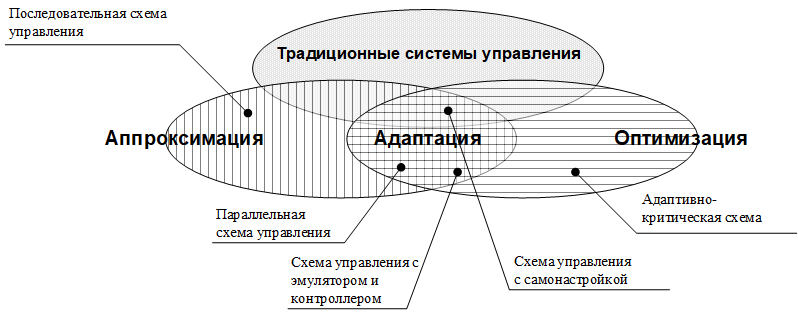
\includegraphics[width=\textwidth]{images/chapter_1/Классификация нейросетевых приемов решения задач управления.png}
    \caption{Классификация нейросетевых приемов решения задач управления}
    \label{fig:neuro_control_classification}
\end{figure}

Рассмотрим более подробно данные подходы к нейросетевому управлению.

\subsection{Последовательная схема управления}

Данная схема наиболее проста, что является как основным достоинством (несмотря на относительную простоту, подходит для решения широкого круга задач), так и недостатком (требует переобучения при изменении параметров объекта управления). Рис. \ref{fig:serial_neuro_control_scheme} отражает данную схему. Являясь одним из самых простых, данный подход имеет множество модификаций \cite{Ruano1992ApplicationsON}. Авторы Woo-Yong Han, Jin-Wook Han и Chang-Goo Lee \cite{Han1999} использовали многослойный персептрон для прогнозирования выхода системы и подстройки затем ПИД-регулятора. Другой коллектив авторов (Corneliu Lazar и др.) использовали подобный подход для надстройки выходы ПИД-регулятора \cite{Lazar2004}. Данная схема также использовалась для управления печью в работе S. Martineau и др. \cite{Martineau2003}.

\begin{figure}[H]
    \centering
    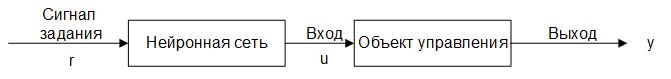
\includegraphics[width=\textwidth]{images/chapter_1/Схема последовательного нейронного управления.png}
    \caption{Схема последовательного нейронного управления}
    \label{fig:serial_neuro_control_scheme}
\end{figure}

\subsection{Схема обратного распространения во времени}

«Обратное распространение во времени» – одна из важных архитектур нейронного управления, использующая алгоритм обратного распространения ошибки. В этой схеме для управления объектом используется две нейронные сети (рис. \ref{fig:neuro_emulator_with_controller}).

\begin{figure}[H]
    \centering
    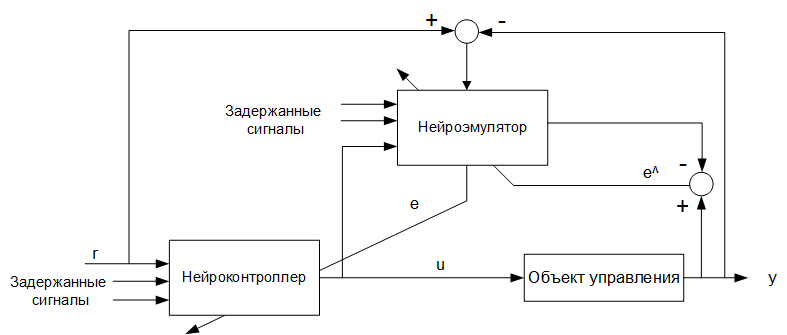
\includegraphics[width=\textwidth]{images/chapter_1/Схема нейронного обучения с эмулятором и контроллером.png}
    \caption{Схема нейронного обучения с эмулятором и контроллером}
    \label{fig:neuro_emulator_with_controller}
\end{figure}

Первая сеть используется как эмулятор, вторая – как контроллер. Сеть эмулятор может обучаться автономно, с использованием архитектуры обобщенного управления, или даже непосредственно, путем ввода случайных входных сигналов для обучения динамике объекта управления.

\subsection{Адаптивно-критическая схема}

Рассматривая подходы к обучению нейросетей, можно отдельно выделить  «обучение с подкреплением» (Reinforcement Learning) или «обучение с критикой». Необходимость применения данной парадигмы возникает в тех случаях, когда известна конечная цель, но неизвестен способ ее достижения. Это тот случай, когда желаемый отклик системы неизвестен, однако может быть дана некоторая оценка ее работы. Такая оценка обычно имеет вид скалярного «подкрепляющего» сигнала. В случае успеха он положителен, при неудаче отрицателен, а в нейтральных случаях равен нулю. Таким образом, можно поощрять за приближение к цели и наказывать за удаление от нее или за медлительность, причем поощрение может быть запаздывающим. Одной из областей применения «обучения с подкреплением» является область задач управления, когда желаемое управление на входе динамического объекта неизвестно, в то время как заметить отклонение его выхода за допустимые пределы несложно. Методы обучения с подкреплением относятся к разряду методов динамического программирования, но без модели объекта. Общая схема приведена на рис. \ref{fig:adaptive_critic_control}.

\begin{figure}[H]
    \centering
    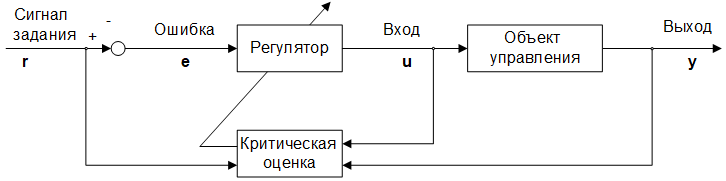
\includegraphics[width=\textwidth]{images/chapter_1/Схема адаптивно-критическая.png}
    \caption{Адаптивно-критическая схема}
    \label{fig:adaptive_critic_control}
\end{figure}

\subsection{Схема управления с самонастройкой}

В данном подходе используется настройка параметров регулятора во время работы системы. Отдельно можно выделить использование ПИД-регулятора с самонастройкой. Он может быть подстроен во время работы за счет изменения его коэффициентов. Существует большое количество схем таких самонастраивающихся ПИД-регуляторов. В данной схеме для настройки коэффициентов  используется нейронная сеть (НС).
Такие нейро-ПИД регуляторы в настоящее время используются для построения различных систем управления \cite{Omatu_Khalid_Yusof}, \cite{Omatu1997}, \cite{Omatu2010}. Рис. \ref{fig:neuro_PID_control} поясняет базовые идеи данного подхода.

\begin{figure}[H]
    \centering
    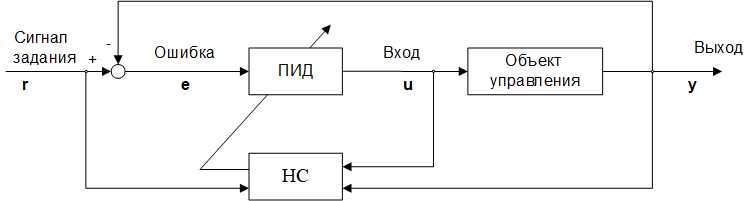
\includegraphics[width=\textwidth]{images/chapter_1/Схема neuroPID общая.png}
    \caption{Схема нейро-ПИД регулятора общая}
    \label{fig:neuro_PID_control}
\end{figure}

Обычно выходом нейронной сети являются коэффициенты ПИД-регулятора. Интересный подход используется в работе Ниша Джха \cite{Nisha2011} – весовые коэффициенты выходного слоя многослойного персептрона соответствуют коэффициентам ПИД-регулятора.

\section{Онтологии и семантические технологии}

В общем случае (отдельно от информационных технологий) слово «семантика» относится к смысловой составляющей языка – значения знаков и структур знаков. При этом семантика противопоставляется синтаксису (формальным правилам соединения знаков в текст). Если речь о семантике заводится в сфере информационных технологий, то имеют в виду особые технологии, архитектуры приложений и языки описания данных, ориентированные на знаковое представление объектов и их свойств в компьютерных моделях предметных областей. В качестве основной цели семантического подхода видится обучение компьютера распознавать смысл данных, описывающих деятельность и ее элементы, то есть реализовать переход от оперирования обезличенными данными к работе со знаниями и значениями. Предполагается, что повсеместное использование семантического подхода в моделировании предметных областей позволит унифицировать обмен информацией между независимыми поставщиками данных и приложениями, а также обеспечит возможность модифицировать структуру данных и бизнес-логику приложений не за счет переписывания кода, а только через преобразование семантически определенных данных. К основным методам семантического подхода следует отнести: унификацию формата записи, уникальную идентификацию записей, включение метаданных в данные, стандартизацию словарей.

Традиционно семантическое описание предметной области именуют онтологией этой области. При этом выражения «онтологическое описание», «онтологическая модель», «онтология предметной области» можно использовать как синонимы. Онтология или онтологическая модель предметной области – это, по сути, структура из сущностей (концептов, понятий, типов объектов), их свойств и правил установления отношений между ними. Обычно онтологию представляют в виде графа, вершинами которого являются объекты, а ребрами – свойства. Часто такую структуру из объектов и значений их свойств, построенную для определенной предметной области, называют графом знаний (Knowledge graph).

\section{Семантические технологии в управлении}

Подход к проектированию различного рода систем на основе онтологических моделей широко используется в настоящее время \cite{Боргест2010}, при этом в особую область исследований выделяют «онтологии предприятия» \cite{Шведин2010}. Суть предлагаемых подходов состоит в построении онтологий, описывающих деятельность того или иного предприятия или его подразделений. В такую систему онтологий при необходимости могут включаться знания различного рода, описывающие тот или иной аспект деятельности предприятия.

Применение онтологического подхода для структуризации знаний предприятия позволяет использовать эти знания более эффективно, в том числе, существенно облегчить процесс модернизации этих знаний, адаптации их под новые задачи, ускорить и упростить процесс обучения нового персонала \cite{Гладун2006}.

В ряде работ рассматриваются применение онтологического подхода для решения конкретных прикладных задач некоторого предприятия \cite{Загорулько2012}.

Однако для существующих онтологических моделей можно выделить ряд общих недостатков:

\begin{itemize}
    \item отсутствие единого подхода к выделению и формированию онтологий, что часто приводит к невозможности интеграции и повторного использования онтологий, разработанных в рамках одного предприятия или даже в рамках разных подразделений одного предприятия;
    \item отсутствие единого подхода к построению иерархии онтологий ограничивает возможность построения комплексной взаимосвязанной системы онтологий, описывающей предприятие на всех необходимых уровнях детализации;
    \item трудности повторного использования онтологий реального предприятия, разработанных другими, из-за их большой сложности;
    \item отсутствие удобных инструментов, поддерживающих разработку и использование онтологий.
\end{itemize}

Для решения данных проблем предлагается использовать описание в виде онтологии стандарта \textbf{ISA-88} - уровень \textbf{SCADA-систем} - на основе технологии \textbf{OSTIS}.

\section{Выводы}

В большинстве работа для «тонкой» подстройки ПИД используется многослойный персептрон (MLP). Также используются рекуррентные или RBF нейронные сети \cite{Reza2011}. Современные подходы основываются на интеграции различных подходов – нечеткой логики \cite{Tahour2007}, генетических алгоритмов \cite{Sharkawy2006}, классических подходов и т.д. \cite{Omatu_Khalid_Yusof}.
Для обучения НС обычно используется алгоритм обратного распространения ошибки (BP algorithm) \cite{Omatu_Khalid_Yusof}, \cite{Ruano1992ApplicationsON} или его модификации \cite{Han1999}. Для поиска начальных значений порогов и весовых коэффициентов используются различные подходы (например, Сигеру Омату \cite{Omatu_Khalid_Yusof} предложил использовать генетические алгоритмы). Для симуляции систем управления широко применяются пакеты MATLAB и Simulink, в некоторых работах можно встретить реализацию в качестве программного модуля для персонального компьютера (PC).

\section{Постановка задачи}

Разработать \textbf{нейро-символический ПИД-регулятор} для использования в проектах АСУТП, также использовать описание в виде онтологии стандарта \textbf{ISA-88} - уровень \textbf{SCADA} - как часть интеллектуальной системы управления, при этом руководствоваться современными подходами \cite{Бурков2022}.
